\documentclass[12pt]{article}
\usepackage{etex}
\reserveinserts{28}

\usepackage{xkeyval}[2005/11/25]
\usepackage{eso-pic}
\usepackage{graphicx}
\usepackage{fp}
\usepackage{tikz}
\usetikzlibrary{calc}
\usetikzlibrary{decorations.pathmorphing}
\usetikzlibrary{decorations.pathreplacing} 
\usetikzlibrary{decorations.shapes} 
\usetikzlibrary{shadows}
\usetikzlibrary{arrows}
\usetikzlibrary{shapes,snakes,shapes.geometric,shapes.misc}
\usepackage{multicol}
\usepackage{arabtex}
\usepackage{amsmath,amsfonts,amssymb}
\usepackage{float}
\usepackage{array,booktabs ,tabularx,multirow}
%\usepackage{euler}
\usepackage[top=1cm,bottom=0cm,left=1cm,right=1cm]{geometry}
\usepackage{fancyhdr}
\usepackage{xlop}
%\usepackage[most]{tcolorbox}
%----------------------------------------...les compteurs..... ----------------------------------------------------------------------%
\newcounter{i}
\setcounter{i}{1}
\newcounter{k}
\setcounter{k}{1}
%----------------------------------------------------------\cadre[x=... ,y=.....,  ]------------------------------------------------------%

% \cadre[			shadow (bool�en),
%					lw = , (�paisseur du trait, en pt)
%					style = , (dashed ou dotted)
%					x = abscisse du sommet en bas � gauche,
%					y = ordonn�e du sommet en bas � gauche,
%					xshadow = d�calage selon x de l'ombre,
%					yshadow = d�calage selon y de l'ombre,
%					color = couleur du cadre,
%					colorshadow = couleur de l'ombre,
%					decoration = nom de la d�coration,
%					doubleline (bool�en) pour pstricks
%				  ]
\makeatletter
\define@cmdkey [PAS] {cadre} {x}{}
\define@cmdkey [PAS] {cadre} {y}{}
\define@cmdkey [PAS] {cadre} {decoration}{}
\define@cmdkey [PAS] {cadre} {shape}{}
\define@cmdkey [PAS] {cadre} {lw}{}
\define@cmdkey [PAS] {cadre} {xshadow}{}
\define@cmdkey [PAS] {cadre} {yshadow}{}
\define@cmdkey [PAS] {cadre} {bordercolor}{}
\define@cmdkey [PAS] {cadre} {incolor}{}
\define@cmdkey [PAS] {cadre} {shadowcolor}{}
\define@cmdkey [PAS] {cadre} {style}{}
\define@boolkey[PAS] {cadre} {shadow}[true]{}
\define@boolkey[PAS] {cadre} {doubleline}[true]{}

\presetkeys    [PAS] {cadre} {	shadow = false,
								lw = 2,
								x = 0.2,
								y = 0.2,
								xshadow =- 0.35,
								yshadow =0.2,
								bordercolor = black,
								incolor = white,
								shadowcolor = gray,
								style = ,
								doubleline = false,
								decoration = , 
								shape = }{}

\newcommand*{\cadre}[1][]{\pasCadre[#1]}

\def\pasCadre[#1]{
	\setkeys[PAS]{cadre}{#1}
	
	\AddToShipoutPicture
	{
		\put(\LenToUnit{\cmdPAS@cadre@x cm},\LenToUnit{\cmdPAS@cadre@y cm})
		{
				\ifPAS@cadre@doubleline
					\edef\dl{double}
				\else
					\edef\dl{}
				\fi
				\begin{tikzpicture}[decoration={\cmdPAS@cadre@decoration,shape=\cmdPAS@cadre@shape}]
					\pgfsetlinewidth{\cmdPAS@cadre@lw pt}
					\ifPAS@cadre@shadow
						\filldraw[
						decorate,
						fill=\cmdPAS@cadre@incolor,
						draw=\cmdPAS@cadre@bordercolor,
						style=\cmdPAS@cadre@style,
						drop shadow={fill=\cmdPAS@cadre@shadowcolor,shadow xshift=\cmdPAS@cadre@xshadow cm,shadow yshift=-\cmdPAS@cadre@yshadow cm},
						\dl] (0,0) -- (0,\paperheight-2*\cmdPAS@cadre@y cm) -- (\paperwidth-2*\cmdPAS@cadre@x cm,\paperheight-2*\cmdPAS@cadre@y cm) -- (\paperwidth-2*\cmdPAS@cadre@x cm,0) -- cycle;
					\else
						\filldraw[
						decorate,
						fill=\cmdPAS@cadre@incolor,
						draw=\cmdPAS@cadre@bordercolor,
						style=\cmdPAS@cadre@style,
						\dl] (0,0) -- (0,\paperheight-2*\cmdPAS@cadre@y cm) -- (\paperwidth-2*\cmdPAS@cadre@x cm,\paperheight-2*\cmdPAS@cadre@y cm) -- (\paperwidth-2*\cmdPAS@cadre@x cm,0) -- cycle;
					\fi
				\end{tikzpicture}
		}
	}
}

\def\nocadre{\ClearShipoutPicture}
%-----------------------------------------------\entete---------------------------------------------------------------------------%
\newcommand{\entete}{
\noindent
\begin{tabularx}{\textwidth}{|r  ||||X|||| r |}
\toprule
\RL{AlmdT AlzmnyT : $1 H$}
&
\centering \RL{{\LARGE Altqwym Alt^sxy.sy }}
&
 \RL{Al-'ism : \hspace{4cm}}\\
 \RL{AldwrT : $I$}& \centering   \RL{\Large{fy m|AdT AlryA.dyAt}}&\RL{Alnq.tT } \\
 \RL{Alm`Aml : $3$} & \centering  \RL{AlsnT Al_tAl_tT 'i`dAdy} & \\
 \bottomrule
\end{tabularx}
}
%-----------------------------------------------
\newcommand{\ExamEntete}{
\noindent
\begin{tabularx}{\textwidth}{||r  ||||X|||| c ||}
\toprule \toprule
\begin{minipage}{0.2\textwidth}
\centering\includegraphics[scale=1]{../images/nourQamar.png}

\begin{arabtext}
AlmdT AlzmnyT : sA`T 

dwrT : ynAyr $2019$

Alm`Aml : $1$
\end{arabtext}
\end{minipage}&
\begin{minipage}{0.4\textwidth}
\begin{center}
 \RL{{\LARGE Alfr.d Almnzly $1$ fy AlryA.ayAt  }}

\RL{\Large{fy mAdT AlryA.dyAt}}

 \RL{AlsnT Al_tAl_tT 'i`dAdy } 
 \end{center}
\end{minipage}&
\begin{minipage}{0.3\textwidth}
\centering\includegraphics[scale=0.5]{images/logo.jpg}
\end{minipage}\\
 \bottomrule  \bottomrule
\end{tabularx}
}
%--\exercice[bareme,bar=...]{........}------------------------------%
\define@cmdkey[EX]{exo}{bar}{}
\define@boolkey[EX]{exo}{bareme}[true]{}
\presetkeys[EX]{exo}{bar= ,bareme=false}{}
\newcommand{\exercice}[2][]{
\setkeys[EX]{exo}{#1}
\setcounter{k}{1}
\tikzstyle{mybox} = [ draw, very thick,rounded corners=3mm, inner sep=10pt, inner ysep=10pt]
\tikzstyle{fancytitle} =[fill=white, text=black,inner ysep=0pt,inner xsep=2pt]
\noindent
\begin{tikzpicture}
\node [mybox] (box){%
    \begin{minipage}{0.88\linewidth}
        #2 
    \end{minipage}
};
\node[fancytitle, right=10pt] at (box.north west) {{\large \LR{Exercice}\arabic{i}}};
\ifEX@exo@bareme
\node[fancytitle] at (box.north){ \cmdEX@exo@bar \LR{pts}};
\fi
\end{tikzpicture}%
\stepcounter{i}
}
%-----------\question[bareme,bar=...]{......}----------------------%
\define@cmdkey[EX]{qst}{bar}{}
\define@boolkey[EX]{qst}{bareme}[true]{}
\presetkeys[EX]{qst}{bar= ,bareme=false}{}
\newcommand{\question}[2][]{
\setkeys[EX]{qst}{#1}
\ifEX@qst@bareme
	\ifdim \cmdEX@qst@bar pt  < 2 pt
\begin{arabtext}
$-\arabic{k}$ \marginpar{ \cmdEX@qst@bar{} pt} #2
\end{arabtext}
	\else
\begin{arabtext}
$-\arabic{k}$ \marginpar{ \cmdEX@qst@bar{} pts} #2
\end{arabtext}
	\fi
\else
\begin{arabtext}
$-\arabic{k}$ #2
\end{arabtext}
\fi
\stepcounter{k}
}
%----------\devoirp[niv=... , num=..., date=..., ds=...]----------%
\define@cmdkey[EX]{devoir}{ds}{}
\define@cmdkey[EX]{devoir}{niv}{}
\define@cmdkey[EX]{devoir}{num}{}
\define@cmdkey[EX]{devoir}{date}{}
\presetkeys[EX]{devoir}{niv=$3$,num=$1$,ds=,date=}{}
\newcommand{\devoir}[1][]{
\setkeys[EX]{devoir}{#1}
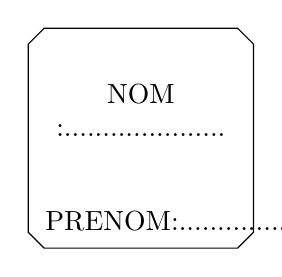
\begin{tikzpicture}
\node [draw,shape=chamfered rectangle] (box1){%
    \begin{minipage}{0.2\textwidth}
    \vspace{0.5cm}
  \center  NOM :.....................
    
   \center PRENOM:...................  
    \end{minipage}
};
\end{tikzpicture}%
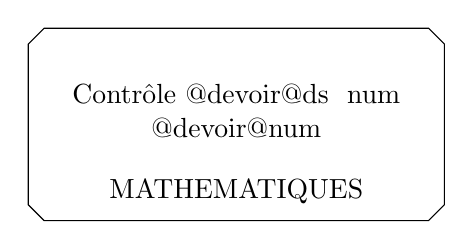
\begin{tikzpicture}
\node [draw,shape=chamfered rectangle] (box2){%
    \begin{minipage}{0.4\textwidth}
    \vspace{0.5cm}
       \center Contrôle \cmdEX@devoir@ds {} num \cmdEX@devoir@num  
           
        \center MATHEMATIQUES
    \end{minipage}
};
\end{tikzpicture}%
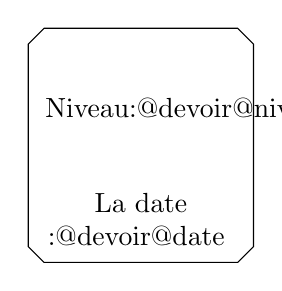
\begin{tikzpicture}
\node [draw,shape=chamfered rectangle] (box3){%
    
    \begin{minipage}{0.2\textwidth}
    \vspace{0.5cm}
    \center\LR{Niveau:{}\cmdEX@devoir@niv  } 
    
      \center  \LR{La date :{}\cmdEX@devoir@date }
    \end{minipage}
};
\end{tikzpicture}%
}
%------------------------------------------------\serie[titre=..]-----------------------------------------------------------------------------%

\define@cmdkey[EX]{serie}{titre}{}
\presetkeys[EX]{serie}{titre=\RL{`nwAn Aldrs}}{}
\newcommand{\serie}[1][]{
\setkeys[EX]{serie}{#1}
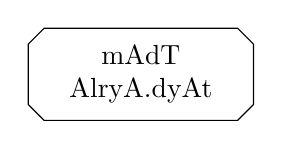
\begin{tikzpicture}
\node [draw,shape=chamfered rectangle] (box1){%
    \begin{minipage}{0.20\textwidth}
       \center\RL{mAdT AlryA.dyAt}
    \end{minipage}
};
\end{tikzpicture}%
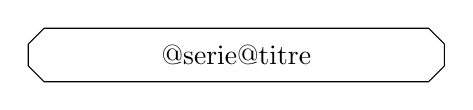
\begin{tikzpicture}
\node [draw,shape=chamfered rectangle] (box2){%
    \begin{minipage}{0.40\textwidth}
      \center\cmdEX@serie@titre
    \end{minipage}
};
\end{tikzpicture}%
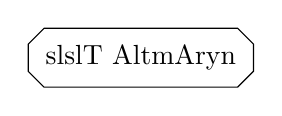
\begin{tikzpicture}
\node [draw,shape=chamfered rectangle] (box3){%
    \begin{minipage}{0.20\textwidth}
   \center\RL{slslT AltmAryn}
    \end{minipage}
};
\end{tikzpicture}%
}
\makeatother
\pagestyle{empty}

\begin{document}
\serie[titre=\RL{mbrhnT .tAlys}]
\begin{multicols}{2}[\RLmulticolcolumns,\raggedcolumns]
\exercice{
\begin{arabtex}
na`tbr Al^skl AltAly .hy_t : $(DE)//(BC)$
\end{arabtex}
\definecolor{cqcqcq}{rgb}{0.7529411764705882,0.7529411764705882,0.7529411764705882}
\begin{tikzpicture}[line cap=round,line join=round,>=triangle 45,x=1.0cm,y=1.0cm]
\clip(-3.02,1.36) rectangle (3.82,5.52);
\draw (0.,5.)-- (-2.,2.);
\draw (-2.,2.)-- (3.,2.);
\draw (3.,2.)-- (0.,5.);
\draw (-1.086153846153846,3.3707692307692305)-- (1.6,3.4);
\draw (-0.86,4.54) node[anchor=north west] {7};
\draw (-1.76,3.02) node[anchor=north west] {3};
\draw (0.06,3.5) node[anchor=north west] {x-1};
\draw (0.02,2.2) node[anchor=north west] {x+1.4};
\begin{scriptsize}
\draw [fill=black] (0.,5.) circle (1.5pt);
\draw[color=black] (0.14,5.28) node {$A$};
\draw [fill=black] (-2.,2.) circle (1.5pt);
\draw[color=black] (-2.22,2.32) node {$B$};
\draw [fill=black] (3.,2.) circle (1.5pt);
\draw[color=black] (3.14,2.28) node {$C$};
\draw [fill=black] (-1.086153846153846,3.3707692307692305) circle (1.5pt);
\draw[color=black] (-1.38,3.64) node {$D$};
\draw [fill=black] (1.6,3.4) circle (1.5pt);
\draw[color=black] (1.74,3.68) node {$E$};
\end{scriptsize}
\end{tikzpicture}

\question{'u.hsb qymT Al`dad $x$}
\question{'i_dA `lmt 'an $EC=4$. 'u.hsb $AE$ .}
}

\exercice{
\begin{arabtext}
lykn $ABC$ m_tl_tA b.hy_t $(BC)//(EF)$ w $AF=4$ w $ EF=5$ w $ BC=9$
\end{arabtext}
\definecolor{cqcqcq}{rgb}{0.7529411764705882,0.7529411764705882,0.7529411764705882}
\begin{tikzpicture}[line cap=round,line join=round,>=triangle 45,x=1.0cm,y=1.0cm] (3.54,6.74);
\clip(-3.5,2.64) rectangle (3.54,6.74);
\draw (-1.,6.)-- (-3.,3.);
\draw (-3.,3.)-- (3.,4.);
\draw (3.,4.)-- (-1.,6.);
\draw (2.02,5.42)-- (-3.04,4.7);
\begin{scriptsize}
\draw [fill=black] (-1.,6.) circle (1.5pt);
\draw[color=black] (-0.84,6.46) node {$A$};
\draw [fill=black] (-3.,3.) circle (1.5pt);
\draw[color=black] (-3.2,3.44) node {$B$};
\draw [fill=black] (3.,4.) circle (1.5pt);
\draw[color=black] (3.14,4.28) node {$C$};
\draw [fill=black] (-1.7436972343522563,4.884454148471615) circle (1.5pt);
\draw[color=black] (-1.98,5.34) node {$E$};
\draw [fill=black] (0.5720615384615388,5.213969230769231) circle (1.5pt);
\draw[color=black] (0.72,5.62) node {$F$};
\end{scriptsize}
\end{tikzpicture}
\question{'u.hsb $AC$ _tm Astntj $FC$ .}
}

\exercice{
\begin{arabtext}
lykn $ABCD$ ^sbh mn.hrf b.hy_t : $(AB)//(CD)$ , Alq.trAn $[AC]$ w $[BD]$ ytqA.t`An fy $I$ , w $IC=5$ w $IB=2$ w $IA=3$ w $AB=4$ 
\end{arabtext}
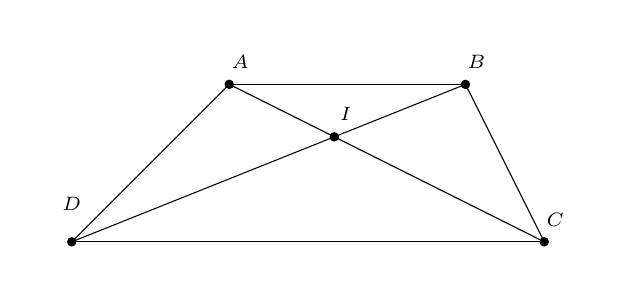
\begin{tikzpicture}[line cap=round,line join=round,>=triangle 45,x=1.0cm,y=1.0cm]
\clip(-4.56,2.56) rectangle (2.78,5.72);
\draw (-2.,5.)-- (1.,5.);
\draw (1.,5.)-- (2.,3.);
\draw (2.,3.)-- (-4.,3.);
\draw (-4.,3.)-- (-2.,5.);
\draw (-2.,5.)-- (2.,3.);
\draw (-4.,3.)-- (1.,5.);
\begin{scriptsize}
\draw [fill=black] (-2.,5.) circle (1.5pt);
\draw[color=black] (-1.86,5.28) node {$A$};
\draw [fill=black] (1.,5.) circle (1.5pt);
\draw[color=black] (1.14,5.28) node {$B$};
\draw [fill=black] (2.,3.) circle (1.5pt);
\draw[color=black] (2.14,3.28) node {$C$};
\draw [fill=black] (-4.,3.) circle (1.5pt);
\draw[color=black] (-4.,3.48) node {$D$};
\draw [fill=black] (-0.6666666666666666,4.333333333333333) circle (1.5pt);
\draw[color=black] (-0.52,4.62) node {$I$};
\end{scriptsize}
\end{tikzpicture}
\question{A.hsb $DC$ w $ID$}
}

\exercice{
\begin{arabtext}
lykn $ABCD$ mtwAzy Al'a.dlA` b.hy_t $(EG) // (BC)$ w $AB=4$ w $AE=1$ w $AC=5$ w $BC=6$
\end{arabtext}
\begin{tikzpicture}[line cap=round,line join=round,>=triangle 45,x=1.0cm,y=1.0cm]
\clip(-3.48,2.36) rectangle (2.76,6.66);
\draw (-3.,6.)-- (1.,6.);
\draw (1.,6.)-- (2.,3.);
\draw (2.,3.)-- (-2.,3.);
\draw (-2.,3.)-- (-3.,6.);
\draw (-2.322,3.966)-- (1.672,3.984);
\draw (-2.,3.)-- (1.,6.);
\begin{scriptsize}
\draw [fill=black] (-3.,6.) circle (1.5pt);
\draw[color=black] (-2.92,6.4) node {$B$};
\draw [fill=black] (1.,6.) circle (1.5pt);
\draw[color=black] (1.14,6.28) node {$C$};
\draw [fill=black] (2.,3.) circle (1.5pt);
\draw[color=black] (2.24,3.28) node {$D$};
\draw [fill=black] (-2.,3.) circle (1.5pt);
\draw[color=black] (-2.4,3.22) node {$A$};
\draw [fill=black] (-2.322,3.966) circle (1.5pt);
\draw[color=black] (-2.66,4.26) node {$E$};
\draw [fill=black] (1.672,3.984) circle (1.5pt);
\draw[color=black] (1.82,4.26) node {$G$};
\draw [fill=black] (-1.0281690140845072,3.9718309859154926) circle (1.5pt);
\draw[color=black] (-1.16,4.4) node {$F$};
\end{scriptsize}
\end{tikzpicture}
\question{A.hsb $AF$ w $EF$ .}
\question{Astntj $FC$ w $FG$ .}
}

\exercice{
\begin{arabtext}
n`tabr Al^skl AltAly .hy_t  $IF= 33$ w $IE=45$ w $IH=30$ w $IG=40$
\end{arabtext}
\definecolor{cqcqcq}{rgb}{0.7529411764705882,0.7529411764705882,0.7529411764705882}
\begin{tikzpicture}[line cap=round,line join=round,>=triangle 45,x=1.0cm,y=1.0cm]
\clip(-4.6,1.38) rectangle (2.68,6.64);
\draw [domain=-4.6:2.68] plot(\x,{(--12.-4.*\x)/4.});
\draw [domain=-4.6:2.68] plot(\x,{(--18.64--1.*\x)/5.02});
\draw [domain=-4.6:2.68] plot(\x,{(-12.48-3.*\x)/-0.58});
\draw [domain=-4.6:2.68] plot(\x,{(--1.12-2.*\x)/-0.44});
\begin{scriptsize}
\draw [fill=black] (-3.,6.) circle (1.5pt);
\draw[color=black] (-2.86,6.28) node {$E$};
\draw [fill=black] (1.,2.) circle (1.5pt);
\draw[color=black] (1.14,2.28) node {$G$};
\draw[color=black] (-4.34,7.64) node {$a$};
\draw [fill=black] (-3.58,3.) circle (1.5pt);
\draw[color=black] (-3.44,3.28) node {$F$};
\draw [fill=black] (1.44,4.) circle (1.5pt);
\draw[color=black] (1.58,4.28) node {$H$};
\draw[color=black] (-5.42,2.98) node {$b$};
\draw[color=black] (-2.48,7.64) node {$c$};
\draw[color=black] (1.96,7.64) node {$d$};
\draw [fill=black] (-0.5946843853820601,3.59468438538206) circle (1.5pt);
\draw[color=black] (-0.46,3.88) node {$I$};
\end{scriptsize}
\end{tikzpicture}
\question{hl AlmstqymAn $(EF)$ w $(GH)$ mtwAzyAn ?}
}

\exercice{
\begin{arabtext}
n`tbr Al^skl AltAly b.hy_t $(BC)//(DE)$ w $(BF)//(DC)$
\end{arabtext}
\definecolor{cqcqcq}{rgb}{0.7529411764705882,0.7529411764705882,0.7529411764705882}
\begin{tikzpicture}[line cap=round,line join=round,>=triangle 45,x=1.0cm,y=1.0cm]
\clip(-4.68,0.98) rectangle (1.3,6.66);
\draw (-2.,6.)-- (-4.,2.);
\draw (-4.,2.)-- (0.54,2.);
\draw (-2.,6.)-- (0.54,2.);
\draw (-3.,2.)-- (-3.,4.);
\draw (-3.,4.)-- (-2.,2.);
\draw (-2.,2.)-- (-2.,6.);
\begin{scriptsize}
\draw [fill=black] (-2.,6.) circle (1.5pt);
\draw[color=black] (-1.86,6.28) node {$D$};
\draw [fill=black] (-4.,2.) circle (1.5pt);
\draw[color=black] (-4.22,1.82) node {$A$};
\draw [fill=black] (0.54,2.) circle (1.5pt);
\draw[color=black] (0.68,2.28) node {$E$};
\draw [fill=black] (-3.,2.) circle (1.5pt);
\draw[color=black] (-2.72,1.76) node {$F$};
\draw [fill=black] (-3.,4.) circle (1.5pt);
\draw[color=black] (-3.22,4.26) node {$B$};
\draw [fill=black] (-2.,2.) circle (1.5pt);
\draw[color=black] (-1.82,1.8) node {$C$};
\end{scriptsize}
\end{tikzpicture}
\question{.hdid Alnsb AlmtsAwyT m`a : $\dfrac{AD}{AB}$}
\question{Astntij 'anna : $AF\times AE=AC^{2}$}
}

\exercice{
\begin{arabtext}
$ADBC$ rbA`y m.hdb ytqA.t` q.trAh $[AB]$ w $[DC]$ fy $E$ b.hy_t $EB=5$ w $AE=3$ w $ED=4$ w $CE=2.4$
\end{arabtext}
\question{'an^sY' Al^skl }
\question{hl AlmstqymAn $(AC)$ w $(BD)$ mtwAzyAn ? m`lilA jwAbk }
\question{hl AlmstqymAn $(AD)$ w $(BC)$ mtwAzyAn ? m`lilA jwAbk}
}

\exercice{
\begin{arabtext}
lykn $ABC$ m_tl_tA w $M$ mnt.sf $[BC]$ , w $(ED)//(AM)$ 'un.zr Al^skl
\end{arabtext}
\definecolor{cqcqcq}{rgb}{0.7529411764705882,0.7529411764705882,0.7529411764705882}
\begin{tikzpicture}[line cap=round,line join=round,>=triangle 45,x=1.0cm,y=1.0cm]
\clip(-4.22,2.08) rectangle (4.14,7.76);
\draw (-1.,6.)-- (-3.,3.);
\draw (-3.,3.)-- (3.,3.);
\draw (-1.,6.)-- (3.,3.);
\draw (-1.,6.)-- (0.,3.);
\draw [domain=-4.22:4.14] plot(\x,{(-0.-3.*\x)/1.});
\draw [domain=-4.22:4.14] plot(\x,{(-21.--3.*\x)/-4.});
\begin{scriptsize}
\draw [fill=black] (-1.,6.) circle (1.5pt);
\draw[color=black] (-0.86,6.28) node {$A$};
\draw [fill=black] (-3.,3.) circle (1.5pt);
\draw[color=black] (-3.22,3.32) node {$B$};
\draw [fill=black] (3.,3.) circle (1.5pt);
\draw[color=black] (3.14,3.28) node {$C$};
\draw [fill=black] (0.,3.) circle (1.5pt);
\draw[color=black] (0.1,2.78) node {$M$};
\draw [fill=black] (-1.,3.) circle (1.5pt);
\draw[color=black] (-1.32,2.8) node {$D$};
\draw[color=black] (-2.88,9.34) node {$e$};
\draw [fill=black] (-1.6666666666666667,5.) circle (1.5pt);
\draw[color=black] (-2.06,5.14) node {$E$};
\draw[color=black] (-5.12,9.34) node {$f$};
\draw [fill=black] (-2.3333333333333335,7.) circle (1.5pt);
\draw[color=black] (-2.1,7.28) node {$F$};
\end{scriptsize}
\end{tikzpicture}
\question{byn 'anna : $\dfrac{DB}{BM}=\dfrac{DE}{AM}$ w $\dfrac{DF}{AM}=\dfrac{DC}{MC}$} 
\question{byn 'anna : $\dfrac{BD}{BM}+\dfrac{DC}{MC}=2$}
\question{bAst`mAl AlntA'ij AlsAbqT byn An : $DE+DF=2AM$}
}

\exercice{
\begin{arabtext}
lykn $EFGH$ ^sbh mn.hrf .hy_t $(EF)//(HG)$ , Almstqym AlmwAzy lilmstqym $(EH)$ w AlmAr mn $F$ yq.t` $(EG)$fy $I$ w yq.t` $(HG)$fy $J$
\end{arabtext}
\definecolor{cqcqcq}{rgb}{0.7529411764705882,0.7529411764705882,0.7529411764705882}
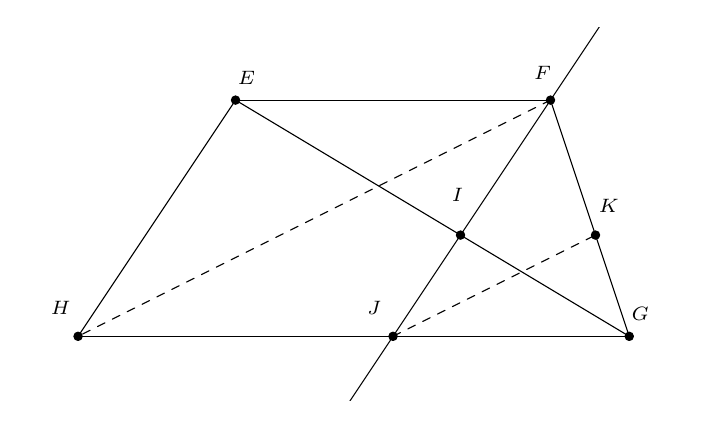
\begin{tikzpicture}[line cap=round,line join=round,>=triangle 45,x=1.0cm,y=1.0cm]
\clip(-5.64,4.18) rectangle (2.72,8.92);
\draw (-3.,8.)-- (1.,8.);
\draw (1.,8.)-- (2.,5.);
\draw (2.,5.)-- (-5.,5.);
\draw (-3.,8.)-- (-5.,5.);
\draw (-3.,8.)-- (2.,5.);
\draw [domain=-5.64:2.72] plot(\x,{(-13.-3.*\x)/-2.});
\draw [dash pattern=on 3pt off 3pt] (1.,8.)-- (-5.,5.);
\draw [dash pattern=on 3pt off 3pt] (-1.,5.)-- (1.5714285714285714,6.285714285714286);
\begin{scriptsize}
\draw [fill=black] (-3.,8.) circle (1.5pt);
\draw[color=black] (-2.86,8.28) node {$E$};
\draw [fill=black] (1.,8.) circle (1.5pt);
\draw[color=black] (0.9,8.34) node {$F$};
\draw [fill=black] (2.,5.) circle (1.5pt);
\draw[color=black] (2.14,5.28) node {$G$};
\draw [fill=black] (-5.,5.) circle (1.5pt);
\draw[color=black] (-5.22,5.36) node {$H$};
\draw[color=black] (2.22,10.3) node {$f$};
\draw [fill=black] (-0.14285714285714285,6.285714285714286) circle (1.5pt);
\draw[color=black] (-0.18,6.8) node {$I$};
\draw [fill=black] (-1.,5.) circle (1.5pt);
\draw[color=black] (-1.24,5.36) node {$J$};
\draw [fill=black] (1.5714285714285714,6.285714285714286) circle (1.5pt);
\draw[color=black] (1.74,6.66) node {$K$};
\end{scriptsize}
\end{tikzpicture}
\question{qArn Alnsbtyn : $\dfrac{IF}{IJ}$ w $\dfrac{IE}{IG}$.}
\question{qArn Alnsbtyn : $\dfrac{KF}{KG}$ w $\dfrac{JH}{JG}$.}
\question{byn 'anna : $(KI)//(JG)$.}

}
\end{multicols}
\end{document}